\section{Execution and deployment.}\label{sec:network}
In section \ref{sec:vlbi} we presented the two operational mode we are
targeting for the software correlator: \emph{batch-execution} and
\emph{real-time}. Batch execution correspond to what the most common
high performance computing scenario. \marginpar{NGHK: Don't
  understand} If we except the \emph{size} of problem described in
Section~\ref{sec:vlbi} and the challenge of making an efficient
distributed application Section~\ref{sec:softwarecorrelation}, we
consider that it is now relatively easy to run \emph{batch} job on top
of existing grids infrastructure and middleware. Running the same
software correlator in a \emph{real-time} mode is much more complex as
the grid infrastructure and corresponding middleware have to provide
guarantees on the Quality of the Service that match the application's
requirement. As these issues are still evolving rapidly we are
testing these aspects of \scarie\ on an experimental grid called DAS-3
and its associated network service called StarPlane.

\subsection{Real-time and quality of service}
The term \emph{real-time} has many definitions in the computer science
community, in this paper we will consider that a \emph{real-time}
computation is a computation in which: \emph{the amount of buffering
  for an infinitely long experiment will only require a finite amount
  of buffers}. This is a formal way to define a process in which the
incoming data are "consumed" by the computation as fast as they are
generated. This definition also imply that once the application is
started the allocated "space" on the resources will be maintained
during the complete execution.

The major resources \scarie\ is using are: the networking bandwidth, 
the computation resource and the disk-space if the data have 
to be saved. The sharing of the computational resource is now
a well understood process. Most of the time it is part of the 
execution service, this service taking a description of the 
application deployment as well as a description of the 
requested service (and resource). The execution service 
allocating rights to access the requested services or 
resource and, finally, if all part of the request 
are fulfilled, deploy the application. 
\begin{figure}
  \centering
  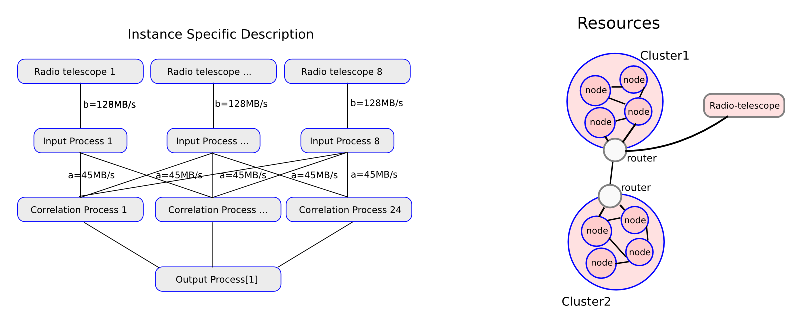
\includegraphics[width=\textwidth]
    {img/mapping.eps}
    \caption{Left: An specific instance of an experiment. Right: The resource set. Resource 
allocation and application scheduling have to map the left side to the resources. }
  \label{fig:mapping}
\end{figure}
The simplest way to offer guaranteed service over a shared resource
can be done restricting the access to only one user at a time. This
approach is used in the DAS-3 grid (based on SGE) in which a node
allocated is simply unusable by other users. Same principle could be
applied to the complete grid including its networks and other
resources. A more complicated, but really interesting approach consist
of sharing the resource under the arbitration of a third party that
will insure that each application is using only the allocated part of
the resource. This is the approach that is often refereed in
bibliography as Layer-2/3 QoS for network services, or the recently
added Completely Fair Scheduler (per application control on their cpu
usage) or IO- (per application IO-bandwith arbitration). In a very
general point of view all these technologies permit to virtualize the
resource thus permit to build on top of a real grid a complete virtual
environment based on user requirements.

\subsection{Running \scarie on \das3 and Starplane}
Networking issues are one of the challenges of the \scarie\ project.
The regular Internet best-effort\marginpar{NGHK: best effort?} Layer3
IP routing has great flexibility but is slow and unpredictable; on the
other hand, dedicated \textit{lightpaths} as available in
\textit{lambda Grids}~\cite{eslea-2007}, with their predictable delays
and throughputs offer good performances and guarantee on the Quality
of Service (QoS). This is the approach that is used in \scarie\ to
delivered the data from the radio-telescope to the computation center.
Giving end user an access to dedicated connection has been implemented
in many of the current research and education networks. The Dutch
National Resarch and Education network SURFnet is one of them.
SURFnet6 deploys multiple fiber optic rings that connect the academic
and research locations around The Netherlands.

For the correlation process we are making experiment on the \das3\
grid\marginpar{NGHK: ??}. The \das3\ supercomputer~\cite{das3} was
deployed in the summer of 2007. It is composed of fives clusters
located in the Netherlands and connected by an photonic network called
StarPlane. StarPlane is also a research project funded by the
Netherlands Organization for Scientific Research (NWO) \emph{and
  carried out at two Dutch Universities: the University of Amsterdam
  (UvA) and the Vrije Universiteit Amsterdam (VU)}\maginpar{NGHK:
  needed}. The goal of the project is to build an
\textit{application-controlled photonic network}. StarPlane manages
eight wavelengths in one of the SURFnet6 optical rings. The novelty of
the StarPlane project lies in its attempt to build a virtual network
service at the lowest possible networking layer. This has the
advantage to improve performances and to dramatically reduce the cost
(the price or the energy) per byte transfered \cite{}\marginpar{TODO}.
A complete virtual network for an application can then be build using
only vlan-on-mac layer 2 switches and layer-1 photonic lighpath. The
other novelty is that the photonic lightpath can dynamically be
reorganized to adapt to the user-application requests.


\subsection{Benchmarks on DAS-3}
\scarie~ and StarPlane have parallel roadmaps. Hence the complete
approach cannot be tested yet. We have conducted correlator
performances test using \das3. The current software correlator is
currently able to perform a 4x128Mbps experiment at 20\% of the
real-time speed using a total of 16 (quad core 2.0Ghz cpu) nodes.

\marginpar{NGHK: relevant?}
In parallel to correlation tests we are working on the real-time
based\marginpar{Real-time based what?}  on the on demand virtual
service. The only part of the StarPlane that is working at the time of
writing is user-requestable lighpath service of StarPlane that permits
to build and allocate a lighpath between two clusters. We tested this
feature by running two client-server applications transmitting data
between cluster. The communication middleware detects this scenario
and allocate a lighpath, while the the lighpath is not available the
application is sending the traffic to the normal network interface;
when it become ready the traffic is switched
\marginpar{automatically?} to the lighpaths.
\begin{figure}[h]
  \centering
  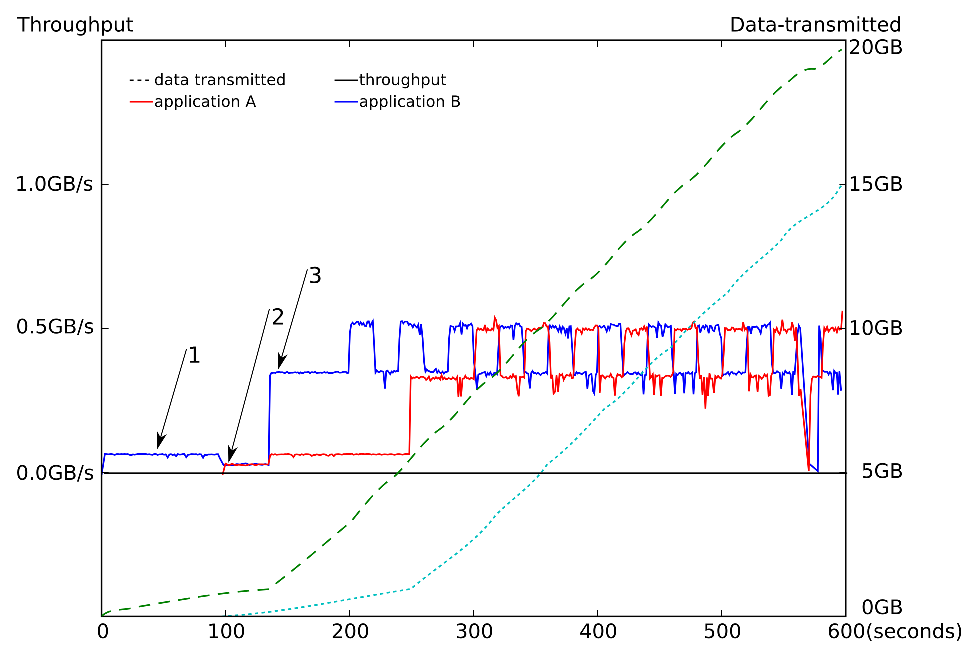
\includegraphics[width=\textwidth] {img/timing.eps}
    \caption{\label{fig:timing}
		Two application executed on the StarPlane network. The application share the ethernet part of the network. Then acquire a lighpath, the change of the bandwith is clearly sensible.}
\end{figure} 

This experiment rise questions, as the supposly secured path that is suppose to deliver reliably "550MB/s" of throughput between a pair of cluster. In Figure~\ref{fig:timing} we can see a periodic artifact, the traffic falling down to 300MB/s for few seconds. A second to investigate issue is that from time to time the lighpath connectivity disapear and these issue have to be investigated in order to provide a "real" guaranteed service. 
